% !TeX spellcheck = en_US
\section{Neural Network Architecture}
In the evolving landscape of NLP, the adaptation of Convolutional Neural Networks on various domains of processing and classification, has marked a significant technological advancement. This transition underscores the versatility of CNNs, which, despite their visual data origins, excel in deciphering the intricate patterns of textual information. The project in discussion exemplifies this innovative application, employing a CNN to tackle a multiclass text classification challenge. Herein, we delve into the architectural choices and strategic decisions underlying the model's design, offering a comprehensive understanding of its construction and functionality. \\
A universal question is wether we must use CNN's or RNN's. The choice between a Convolutional Neural Network (CNN) and a Recurrent Neural Network (RNN) depends on the specific task and the nature of our data. \\

In general, RNN is a class of artificial neural network where connections between nodes form a directed graph along a sequence. It is basically a sequence of neural network blocks that are linked to each other like a chain. Each one is passing a message to a successor. This architecture allows RNN to exhibit temporal behavior and capture sequential data which makes it a more ‘natural’ approach when dealing with textual data since text is naturally sequential. RNNs usually are good at predicting what comes next in a sequence\\

Controversely, CNN is a class of deep, feed-forward artificial neural networks where connections between nodes do not form a circle. CNNs are basically just several layers of convolutions with nonlinear activation functions like ReLU or tanh applied to the results. In a traditional feedforward neural network we connect each input neuron to each output neuron in the next layer. That’s also called a fully connected layer. In CNNs we don’t do that. Instead, we use convolutions over the input layer to compute the output. This results in local connections, where each region of the input is connected to a neuron in the output. Each layer applies different filters, typically hundreds or thousands like the ones shown below, and combines their results. CNNs can learn to classify a sentence or a paragraph.\\

An RNN is trained to recognize patterns across time, while a CNN learns to recognize patterns across space. The best way to determine which to use is to try both and see which one performs better on our project. \\
A big argument for CNNs is that they are exceptionaly fast. Based on computation time, CNN's seems to be much faster, sometimes also 5 times faster, than RNN's.
 











We knew from the start that 

\begin{minipage}{0.48\linewidth}
	\centering
	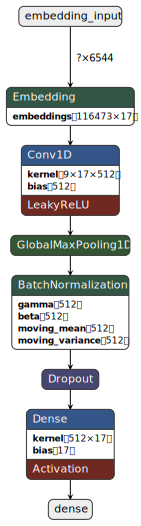
\includegraphics[height=0.9\textheight]{Images/model_level_1.keras.pdf}
	\captionof{figure}{}
\end{minipage}\hfill
\begin{minipage}{0.48\linewidth}
	\centering
	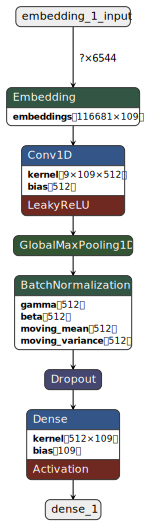
\includegraphics[height=0.9\textheight]{Images/model_level_2.keras.pdf}
	\captionof{figure}{}
\end{minipage}